%TITULO------------------------------------------------------------------------

%==============================================================================
\chapter[Análise de Estabilidade do Alg. Adaptativo]{Análise de Estabilidade
    Robusta do Algoritmo Adaptativo}\label{provas}
%==============================================================================

\section{Descrição da Planta e do Modelo de Referência}

    Considere a planta SISO, LTI
    %
    \begin{equation}
        y(k) = G(z) \cdot u(k) = G_o(z) \cdot u(k) + \Delta(z) \cdot u(k)\text{,}
        \label{eq:saida_da_planta}
    \end{equation}
    %
    onde:
    %
    \begin{equation}
        G_o(z) = k_p \frac{Z_o(z)}{P_o(z)}\text{.}
    \end{equation}

    $G(z)$ é uma função de transferência estritamente própria, $Z_o(z)$ e $P_o(z)$
    são polinômios mônicos e o sinal do ganho $k_p$ é assumido como sendo conhecido. Além
    disso, o comportamento desejado da planta em malha fechada é descrito por um modelo de
    referência, dado pela função de transferência
    %
    \begin{equation}
        y_m(k) = W_m(z) \cdot r(k) = \frac{k_m}{P_m(z)} r(k)\text{,}
        \label{eq:saida_do_modelo_de_referencia}
    \end{equation}
    %
    onde $P_m(z)$ é um polinômio mônico e $k_m > 0$.

    O objetivo do Controle por Modelo de Referência ou MRC (do inglês \emph{Model
    Reference Control}) é determinar a entrada $u$ da planta de forma que sua saída
    $y$ rastreie a saída do modelo de referência $y_m$ tão próximo quanto possível,
    desde que mantendo os sinais de malha fechada limitados.

    É necessário definir uma Lei de Controle e uma Lei de Adaptação Paramétrica para
    projetar a entrada $u$ da planta.

    Caso existam incertezas paramétricas, utiliza-se uma técnica de controle adaptativo
    que resulta no Controlador Adaptativo por Modelo de Referência ou MRAC (do inglês
    \emph{Model Reference Adaptive Control}). É necessário definir uma Lei de Controle
    e uma Lei de Adaptação Paramétrica para projetar a entrada $u$ da planta. No caso de
    plantas com dinâmicas não-modeladas, é necessário modificar a lei de adaptação
    paramétrica de forma a garantir a robustez do controlador. Neste caso, diz-se que o
    controlador é MRAC robusto.

    As hipóteses feitas sobre a planta e o modelo de referência são as seguintes:

    \begin{itemize}
        \item[] $H_1$) $Z_o(z)$ é um polinômio mônico, Schur de grau $m$ conhecido;
        \item[] $H_2$) $P_o(z)$ é mônico de grau $n$ conhecido e $n^* = n - m \geq 1$ é o grau
            relativo da planta nominal $G_o(z)$;
        \item[] $H_3$) São conhecidos o sinal do ganho $k_p$ e o limite superior de $|k_p|$,
            $k_{p0} \geq |k_p|$;
        \item[] $H_4$) $\Delta(z)$ é uma função de transferência estável e estritamente
            própria;
        \item[] $H_5$) É conhecido um limite superior $\delta_0 \in (0, \, 1)$ tal que
            $\Delta(z)$ possui todos os seus pólos confinados num círculo aberto de
            raio $|z| \geq \sqrt{\delta_0}$;
        \item[] $H_6$) $P_m(z)$ é um polinômio mônico, Schur de grau $n^*$.
    \end{itemize}

    As hipóteses $H_1$, $H_2$ e $H_3$ são necessárias para garantir a estabilidade do
    controlador projetado e para o projeto do ganho da lei de adaptação paramétrica.
    As hipóteses $H_4$ e $H_5$ são necessárias para garantir a limitação dos sinais
    de malha fechada e a robustez da lei de adaptação paramétrica. A hipótese $H_6$
    é usada para a escolha de um modelo de referência adequado.

\section{Estrutura do Algoritmo Adaptativo}

    Em casos onde os estados da planta não são medidos é possível a utilização de
    estimadores, de onde resulta a estrutura para a lei de
    controle~\cite{ref:TAO}
    %
    \begin{equation}
        u = \theta^T \omega\text{,}
    \end{equation}
    %
    na qual os vetores $\theta$ e $\omega$ são definidos como
    %
    \begin{equation}
        \begin{split}
            \theta^T & = \left[ \begin{matrix} \theta_1^T, & \theta_2^T, & \theta_3, & \theta_4
                \end{matrix} \right]\text{ e}\\
            \omega & = {\left[ \begin{matrix} \omega_1 & \omega_2 & y & r \end{matrix}
                \right]}^T\text{.}
        \end{split}
    \end{equation}

    A Fig.~\ref{fig:cascata} apresenta a estrutura geral do sistema de controle.

    \begin{figure}[htb]
        \centering{
            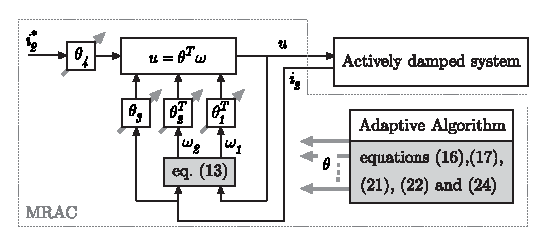
\includegraphics[width=0.9\textwidth]{img/adaptive_block_diagram}}
        \renewcommand\figurename{Fig.}
        \caption{Estrutura do controlador MRAC.}
        \label{fig:cascata}
    \end{figure}

    A entrada $u$ e a saída $y$ da planta são usadas para gerar os sinais $\omega_1$ e
    $\omega_2$ dados por
    %
    \begin{equation}
        %\begin{split}
            \omega_1(k) = \frac{\alpha(z)}{\Lambda(z)} u(k) \text{ e }
            \omega_2(k) = \frac{\alpha(z)}{\Lambda(z)} y(k)
        %\end{split}
        \label{eq:omega_1_2}
    \end{equation}
    %
    com $\Lambda(z)$ estável e $\alpha(z)$ dados por
    %
    \begin{equation*}
        \alpha(z) = \left[ \begin{matrix} z^{n-2}, & ..., & z, & 1 \end{matrix} \right]
        \text{ e }
        \Lambda(z) = z^{n-1} + \lambda_{n-2} z^{n-2} + ... + \lambda_1 z + \lambda_0\text{.}
    \end{equation*}

    Nota-se que a dimensão de $\alpha$ e $\Lambda$ é definida com base no grau da planta.
    Considerando que a planta $G(z)$ pode ser descrita em termos de uma parte conhecida
    $G_o(z)$ e uma parte com dinâmicas não-modeladas do tipo aditiva, estável e estritamente
    própria $\Delta(z)$ tem-se
    %
    \begin{equation}
        G(z) = G_o(z) + \Delta(z) \text{.}
        \label{eq:planta_go_delta}
    \end{equation}

    Define-se o modelo de referência como sendo
    %
    \begin{equation*}
        y_m = W_m(z) r \text{.}
    \end{equation*}

    É necessário garantir que o grau relativo da planta $G_o(z)$ e do modelo de referência
    $W_m(z)$ sejam iguais para que seja possível resolver a condição de casamento
    \cite{ref:IOANNOU}. Dessa forma, garante-se que existe um conjunto de ganhos
    $\theta = \theta^*$ tal que a saída da planta $y$ é igual a saída do modelo de referência
    $y_m$ quando $\Delta(z) = 0$.

    Para a obtenção dos sinais necessários para a implementação do controlador adaptativo,
    parte-se da definição da lei de controle assumindo a existência de um conjunto de ganhos
    $\theta = \theta^*$. Assim
    %
    \begin{equation}
        \begin{split}
            u(k) &= \theta^T \omega = \theta^T \omega + \theta^{*T} \omega - \theta^{*T} \omega\\
            u(k) &= \phi^T \omega + \theta^{*T} \omega
            \label{eq:u_para_theta_estrela}
        \end{split}
    \end{equation}
    %
    onde:
    %
    \begin{equation*}
        \phi = \theta - \theta^* \text{.}
    \end{equation*}
    %
    De (\ref{eq:u_para_theta_estrela}):
    %
    \begin{equation*}
        u(k) = \phi^T \omega + \theta_1^{*T} \omega_1 + \theta_2^{*T} \omega_2 + \theta_3^* y(k)
            + \theta_4 r \text{.}
    \end{equation*}
    %
    Considerando (\ref{eq:omega_1_2}) tem-se
    %
    \begin{equation*}
        u(k) = \phi^T \omega + \theta_1^{*T} \frac{\alpha(z)}{\Lambda(z)} u(k) +
            \left( \theta_2^{*T} \frac{\alpha(z)}{\Lambda(z)} + \theta_3^* \right)
            y(k) + \theta_4^* r \text{.}
    \end{equation*}
    %
    Definindo
    %
    \begin{equation*}
        \begin{split}
            F_1 &= \theta_1^{*T} \frac{\alpha(z)}{\Lambda(z)}\\
            F_2 &= \theta_2^{*T} \frac{\alpha(z)}{\Lambda(z)} + \theta_3^*
        \end{split}
    \end{equation*}
    %
    e considerando que $y(k) = G(z) u(k)$, obtém-se
    %
    \begin{equation}
        \left( 1 - F_1(z) - F_2(z) G(z) \right) u(k) = \phi^T \omega + \theta_4^* r \text{.}
        \label{eq:funcao_de_fs}
    \end{equation}

    Levando em conta que, na ausência de dinâmicas não modeladas, existe um conjunto de
    ganhos $\theta = \theta^*$ tal que $\phi = 0$ e $y = y_m$, têm-se:
    %
    \begin{equation}
        y(k) = G_o(z) u(k) = y_m = W_m(z) r
    \end{equation}
    %
    Então de (\ref{eq:funcao_de_fs}):
    %
    \begin{equation}
        \left( 1 - F_1(z) - F_2(z) G(z) \right) u(k) = \theta_4^* r
    \end{equation}
    %
    Como $r = W_m(z)^{-1} y_m$, e definindo $\rho^* = 1/\theta_4^*$:
    %
    \begin{equation*}
        \rho^* W_m(z) \left( 1 - F_1(z) - F_2(z) G(z) \right) u(k) = y_m = G_o(z) u(z)
    \end{equation*}
    %
    O que resulta em:
    %
    \begin{equation}
        G_o(z) = \rho^* W_m(z) \left( 1 - F_1(z) - F_2(z) G(z) \right)
        \label{eq:go_z_em_funcao_de_f}
    \end{equation}
    %
    De (\ref{eq:saida_da_planta}) e (\ref{eq:go_z_em_funcao_de_f}) resulta:
    %
    \begin{equation*}
        \left[ 1 - F_1(z) - F_2(z) \left( G_o(z) + \Delta(z) \right) \right] u(k) =
            \phi^T \omega + \theta_4^* r
    \end{equation*}
    %
    \begin{equation}
        \left( 1 - F_1(z) - F_2(z) G_o(z) \right) u(k) = \phi^T \omega + \theta_4^* r +
            F_2(z) \Delta(z) u(k)
        \label{eq:phi_theta_f}
    \end{equation}
    %
    Substituindo (\ref{eq:go_z_em_funcao_de_f}) em (\ref{eq:saida_da_planta}), obtém-se
    %
    \begin{equation}
        y(k) = \rho^* W_m(z) \left( 1 - F_1(z) - F_2(z) G_o(z) \right) u(k) + \Delta(z)
            u(k) \text{.}
        \label{eq:y_em_funcao_f}
    \end{equation}
    %
    Substituindo (\ref{eq:phi_theta_f}) em (\ref{eq:y_em_funcao_f}) resulta
    %
    \begin{equation*}
        y(k) = \rho^* W_m(z) \left[ \phi^T \omega + \theta_4^* r + F_2(z) \Delta(z) u(k) \right]
            + \Delta(z) u(k) \text{ ou }
    \end{equation*}
    %
    \begin{equation*}
        y(k) = \rho^* W_m(z) \left[ \phi^T \omega + \theta_4^* r \right] + \left( \rho^* W_m(z)
            \cdot F_2(z) + 1 \right) \cdot \Delta(z) u(k) \text{.}
    \end{equation*}
    %
    Definindo
    %
    \begin{equation*}
        \bar{\Delta}(z) = \left( \rho^* W_m(z) F_2 + 1 \right) \Delta(z)
    \end{equation*}
    %
    também
    %
    \begin{equation*}
        \eta(k) = \bar{\Delta}(z) u(k)
    \end{equation*}
    %
    tem-se que:
    %
    \begin{equation*}
        y(k) = \rho^* W_m(z) \left[ \phi^T(k) \omega(k) + \theta_4^* r(k) \right] + \eta(k)
        %\label{eq:y_em_funcao_de_eta}
    \end{equation*}
    %
    com $y_m(k) = W_m(z) r(k)$ e $\rho^* = 1/\theta_4^*$:
    %
    \begin{equation}
        e_1(k) = y(k) - y_m(k) = \rho^* W_m(z) \left[ \phi^T(k) \omega(k) \right] + \eta(k) \text{.}
        \label{eq:e1_em_funcao_de_eta}
    \end{equation}

    Para sistemas discretos não se pode garantir que $W_m(z)$ será estritamente positivo e real
    (\emph{SPR}), não sendo possível a utilização do erro tal como dado em
    (\ref{eq:e1_em_funcao_de_eta}) para o projeto da lei de adaptação paramétrica, visto que
    não é possível provar que o algoritmo resultante é estável. Portanto, define-se uma equação
    de erro aumentado $e_a$ para o qual será possível demonstrar a estabilidade do algoritmo.
    O erro aumentado é dado por
    %
    \begin{equation}
        e_a = \rho^* \phi^T \zeta + \tilde{\rho} \cdot e_2 + \eta
        \label{eq:ea_erro_aumentado}
    \end{equation}
    %
    onde:
    %
    \begin{itemize}[leftmargin=+2cm]
        \item[] $e_2$ é o sinal de aumento do erro;
        \item[] $\tilde{\rho}$ é o erro na estimação da divisão do ganho da planta
            pelo ganho do modelo de referência;
        \item[] $\zeta(k) = W_m(z) \omega(k) \text{.}$
    \end{itemize}
    %
    %E:
    %
    %\begin{equation}
    %    \zeta(k) = W_m(z) \cdot \omega(k)
    %    \label{eq:zeta}
    %\end{equation}

    Para a implementação, é possível expressar o erro aumentado em uma forma computável:
    %
    \begin{equation}
        e_a = e_1 + \rho \cdot e_2
        \label{eq:erro_aumentado_computavel}
    \end{equation}
    %
    A partir de (\ref{eq:ea_erro_aumentado}) pode-se obter o seguinte algoritmo de adaptação
    paramétrica
    %
    \begin{equation}
        \begin{split}
            \theta(k+1) &= \theta(k) - \mathrm{sgn}(k_p) \gamma_d \frac{\zeta(k) \cdot e_a(k)}{{\bar{m}}^2(k)} \\
            \rho(k+1) &= \rho(k) - \gamma \frac{e_2(k) \cdot e_a(k)}{{\bar{m}}^2(k)} \\
            {\bar{m}}^2 &= m^2(k) + \zeta^T(k) \zeta(k) + {e_2}^2(k) \\
            m^2(k+1) &=  \delta_0(m^2(k) - 1) + u^2(k) + y^2(k) + 1
        \end{split}
        \label{eq:equacoes_algoritmo_adaptativo}
    \end{equation}
    %
    onde:
    %
    \begin{itemize}[leftmargin=+2cm]
        \item[] $\gamma$ e $\gamma_d$ são ganhos das leis de adaptação, e
        \item[] $\delta_0$ é uma constante utilizada no normalizador para o projeto
            da robustez das leis de adaptação.
    \end{itemize}

\section{Análise de Estabilidade Robusta}

    Considerando uma função definida positiva:

    \begin{equation}
        \begin{split}
            V(k) = \frac{|\rho^*|}{\gamma_d} \phi^T(k) \phi(k) + \frac{1}{\gamma} {\tilde{\rho}}^2(k) \\
            \Delta V(k) = V(k+1) - V(k) \leq 0
        \end{split}
    \end{equation}

    Isto é:

    \begin{equation}
        \Delta V(k) = \frac{|\rho^*|}{\gamma_d} \phi^T(k+1) \phi(k+1) - \frac{|\rho^*|}{\gamma_d} \phi^T(k) \phi(k)
            + \frac{1}{\gamma} {\tilde{\rho}}^2(k+1) - \frac{1}{\gamma} {\tilde{\rho}}^2(k)
        \label{eq:delta_v}
    \end{equation}

    Como $\phi = \theta - \theta^*$ e $\tilde{\rho} = \rho - \rho^*$:

    \begin{equation}
        \phi(k+1) = \phi(k) - \mathrm{sgn}(k_p) \gamma_d \frac{\zeta(k) \cdot e_a(k)}{{\bar{m}}^2(k)}
        \label{eq:phi_k1}
    \end{equation}

    \begin{equation}
        \tilde{\rho}(k+1) = \tilde{\rho}(k) - \gamma \frac{e_2(k) \cdot e_a(k)}{{\bar{m}}^2(k)}
        \label{eq:tilde_rho_k1}
    \end{equation}

    Substituindo (\ref{eq:phi_k1}) e (\ref{eq:tilde_rho_k1}) em (\ref{eq:delta_v}), obtém-se:

    \begin{equation}
        \begin{split}
            \Delta V(k) &= \frac{|\rho^*|}{\gamma_d} \left[ \phi^T(k) - \mathrm{sgn}(k_p) \gamma_d
                \frac{\zeta^T(k) \cdot e_a(k)}{{\bar{m}}^2(k)} \right] \cdot
                \left[ \phi(k) - \mathrm{sgn}(k_p) \gamma_d \frac{\zeta(k) \cdot e_a(k)}{{\bar{m}}^2(k)} \right] \\
                &\qquad {}- \frac{|\rho^*|}{\gamma_d} \phi^T(k) \phi(k) + \frac{1}{\gamma} \left[ \tilde{\rho}(k)
                - \gamma \frac{e_2(k) \cdot e_a(k)}{{\bar{m}}^2(k)} \right]
                - \frac{1}{\gamma} {\tilde{\rho}}^2(k)
        \end{split}
    \end{equation}

    Que pode ser simplificado para:

    \begin{equation*}
        \begin{split}
            \Delta V(k) &= |\rho^*| \left[ - 2 \cdot \mathrm{sgn}(k_p) \cdot e_a(k) \frac{\phi^T(k) \zeta(k)}{{\bar{m}}^2(k)}
            + \gamma_d \cdot {e_a}^2(k) \frac{\zeta^T(k) \zeta(k)}{{\bar{m}}^2(k) \cdot {\bar{m}}^2(k)} \right] \\
            &\qquad {}- 2 \cdot e_2(k) \cdot \frac{\bar{\rho}(k) \cdot e_1(k)}{{\bar{m}}^2(k)}
            + \gamma \frac{{e_2}^2(k) \cdot {e_a}^2(k)}{{\bar{m}}^2(k) \cdot {\bar{m}}^2(k)}
        \end{split}
    \end{equation*}

    Que pode ser reescrito como:

    \begin{equation*}
        \begin{split}
            \Delta V(k) &= -2 \cdot \mathrm{sgn}(k_p) |\rho^*| e_a(k) \frac{\phi^T(k) \cdot \zeta(k)}{{\bar{m}}^2(k)}
                -2 \cdot e_2(k) \frac{\tilde{\rho}(k) \cdot e_a(k)}{{\bar{m}}^2(k)} \\
                &\qquad {}+ \left( |\rho^*| \gamma_d \frac{\zeta^T(k) \cdot \zeta(k)}{{\bar{m}}^2(k)}
                + \gamma \frac{{e_2}^2(k)}{{\bar{m}}^2(k)} \right) \frac{{e_a}^2}{{\bar{m}}^2(k)}
            \end{split}
    \end{equation*}

    Levando em conta que $\mathrm{sgn}(k_p)\cdot|\rho^*|=\rho^*$ e introduzindo um termo ${}+ \eta - \eta$, obtém-se:

    \begin{equation*}
        \begin{split}
            \Delta V(k) &= -2 \frac{e_a(k)}{{\bar{m}}^2(k)} \left[ \rho^* \phi^T(k) \zeta(k)
                + \tilde{\rho}(k) e_2(k) + \eta - \eta \right] \\
                &\qquad {}+ \left( |\rho^*| \gamma_d \frac{\zeta^T(k) \cdot \zeta(k)}{{\bar{m}}^2(k)}
                + \gamma \frac{{e_2}^2(k)}{{\bar{m}}^2(k)} \right) \frac{{e_a}^2}{{\bar{m}}^2(k)}
        \end{split}
    \end{equation*}

    Considerando que $e_a(k) = \rho^* \cdot \phi^T(k) \zeta(k) + \tilde{\rho}(k) \cdot e_2(k) + \eta$, obtém-se:

    \begin{equation*}
        \Delta V(k) = -2 \frac{e_a(k)^2}{{\bar{m}}^2(k)} +2 \frac{e_a(k)}{{\bar{m}}^2(k)} \eta
            + \left( |\rho^*| \gamma_d \frac{\zeta^T(k) \cdot \zeta(k)}{{\bar{m}}^2(k)}
            + \gamma \frac{{e_2}^2(k)}{{\bar{m}}^2(k)} \right) \frac{{e_a}^2}{{\bar{m}}^2(k)}
    \end{equation*}

    Que pode ser reescrito como:

    \begin{equation*}
        \Delta V(k) = - \left( 1 - \frac{|\rho^*| \gamma_d \zeta^T(k) \cdot \zeta(k)
            + \gamma {e_2}^2(k)}{{\bar{m}}^2(k)} \right) \frac{{e_a}^2(k)}{{\bar{m}}^2}
            + 2 \frac{e_a(k) \cdot \eta}{{\bar{m}}^2} - \frac{{e_a}^2(k)}{{\bar{m}}^2}
    \end{equation*}

    Que, por sua vez, pode ser reescrito como:

    \begin{equation}
        \begin{split}
            \Delta V(k) &= - \left( 1 - \frac{|\rho^*| \gamma_d \zeta^T(k) \cdot \zeta(k)
            + \gamma {e_2}^2(k)}{{\bar{m}}^2(k)} \right) \frac{{e_a}^2(k)}{{\bar{m}}^2} \\
            &\qquad {}- {\left( \frac{e_a(k)}{\bar{m}} - \frac{\eta}{\bar{m}} \right)}^2 + \frac{\eta^2}{{\bar{m}}^2}
        \end{split}
    \end{equation}

    \begin{teorema}
        A estrutura de controle (\ref{eq:saida_do_modelo_de_referencia}) - (\ref{eq:omega_1_2}) e
        (\ref{eq:erro_aumentado_computavel}) com o algoritmo adaptativo
        (\ref{eq:equacoes_algoritmo_adaptativo}) garante a limitação dos seguintes sinais na malha
        fechada~\cite{ref:STEFANELLO}:

        \begin{itemize}
            \item[] i) $|\eta|/m \leq \Delta_0$ onde $\Delta_0 \in \mathcal{L}_{\infty}$;
            \item[] ii) $e_a/\bar{m}$, $e_am/{\bar{m}}^2$, $e_a/{\bar{m}}^2 \in \mathcal{S}
                \left( {\Delta_0}^2/h^2 \right)$ e $h \in (0, 1)$;
            \item[] iii) $|\Delta\theta_i(k)| \in \mathcal{S}\left(\left(\gamma_d + \lambda\gamma_s\right)^2
                {\Delta_0}^2/h^2 \right) \forall k > 0, i=1, \ldots, 2n_0$ onde $\Delta\theta_i(k) = \theta_i(k)
                - \theta_i(k-1)$ e $h \in (0, 1)$;
            \item[] iv) $||\omega_1||/m$, $||\omega_2||/m \in \mathcal{L}_{\infty}$;
            \item[] v) $|y|/m$, $|u|/m \in \mathcal{L}_{\infty}$;
            \item[] vi) $||\omega||/m \in \mathcal{L}_{\infty}$;
            \item[] vii) $||\zeta||/m \in \mathcal{L}_{\infty}$;
            \item[] viii) $e_2/m \in \mathcal{L}_{\infty}$;
            \item[] ix) $m^2(k+1)/m^2(k) \in \mathcal{L}_{\infty}$.
        \end{itemize}
    \end{teorema}

    %falta escrever que, atendida a relação entre gamma e gamma_d, os outros termos são funções de
    %termos quadráticos, isto é, serão sempre de sinal negativo. Falta ver com o márcio como eu explico
    %que a influência do terceiro termo, eta^2/m^2, é negligenciável. Depois disto, está pronto.


%FIM---------------------------------------------------------------------------
